According to the methodology described in Chapter \ref{chap:methodology}, we ran a set of experiments
for each of the tasks described in Section \ref{sec:tasks}.
Each experiment is composed of a training phase and a testing phase:

\begin{itemize}
	\item Training phase: The agent is actively learning by sampling data from the simulation server to 
	actively update the parameters of the policy (represented by a neural network).
	\item Evaluation phase: After the initial learning phase, we freeze all the parameters of the agent's 
	policy and evaluate how well it does on the task at hand. 
	We use the metrics describes in Section \ref{sec:metrics} to quantify how well the agent is able to learn the task.
\end{itemize}

In the training phase, we compare the performance for three different deep reinforcement learning algorithms for continuous
control: DDPG, TRPO and PPO.
After the training phase is complete, we evaluate the performance of the learned behaviors and compare them with
classical control behaviors developed by the ITAndroids teams that serve as a performance baseline.

We ran all experiments on a Intel i7-7500U CPU with $4$ logical cores and a GeForce 940MX integrated GPU.
It is important to notice that physical simulation is CPU-bound and, therefore, CPU is the leading
factor of how long the training phase takes to complete.
We will now describe the experiments for each of the tasks.

\section{Humanoid Speed Walker (Warm-Up) Task}

In this domain we are only interested in getting familiar with the environment by learning a very simple task.
We ran PPO once for $10^6$ timesteps with the parameters described in Appendix \ref{chap:appendix_experiment}.
Figure \ref{fig:constant_episode_rew} shows how the average episode returns changes during the training phase of
the algorithm.
Notice how the average episode reward is consistently increasing showing clear signs that the agent is learning how to walk
with the reference speed.

\begin{figure}[ht]
	\centering
	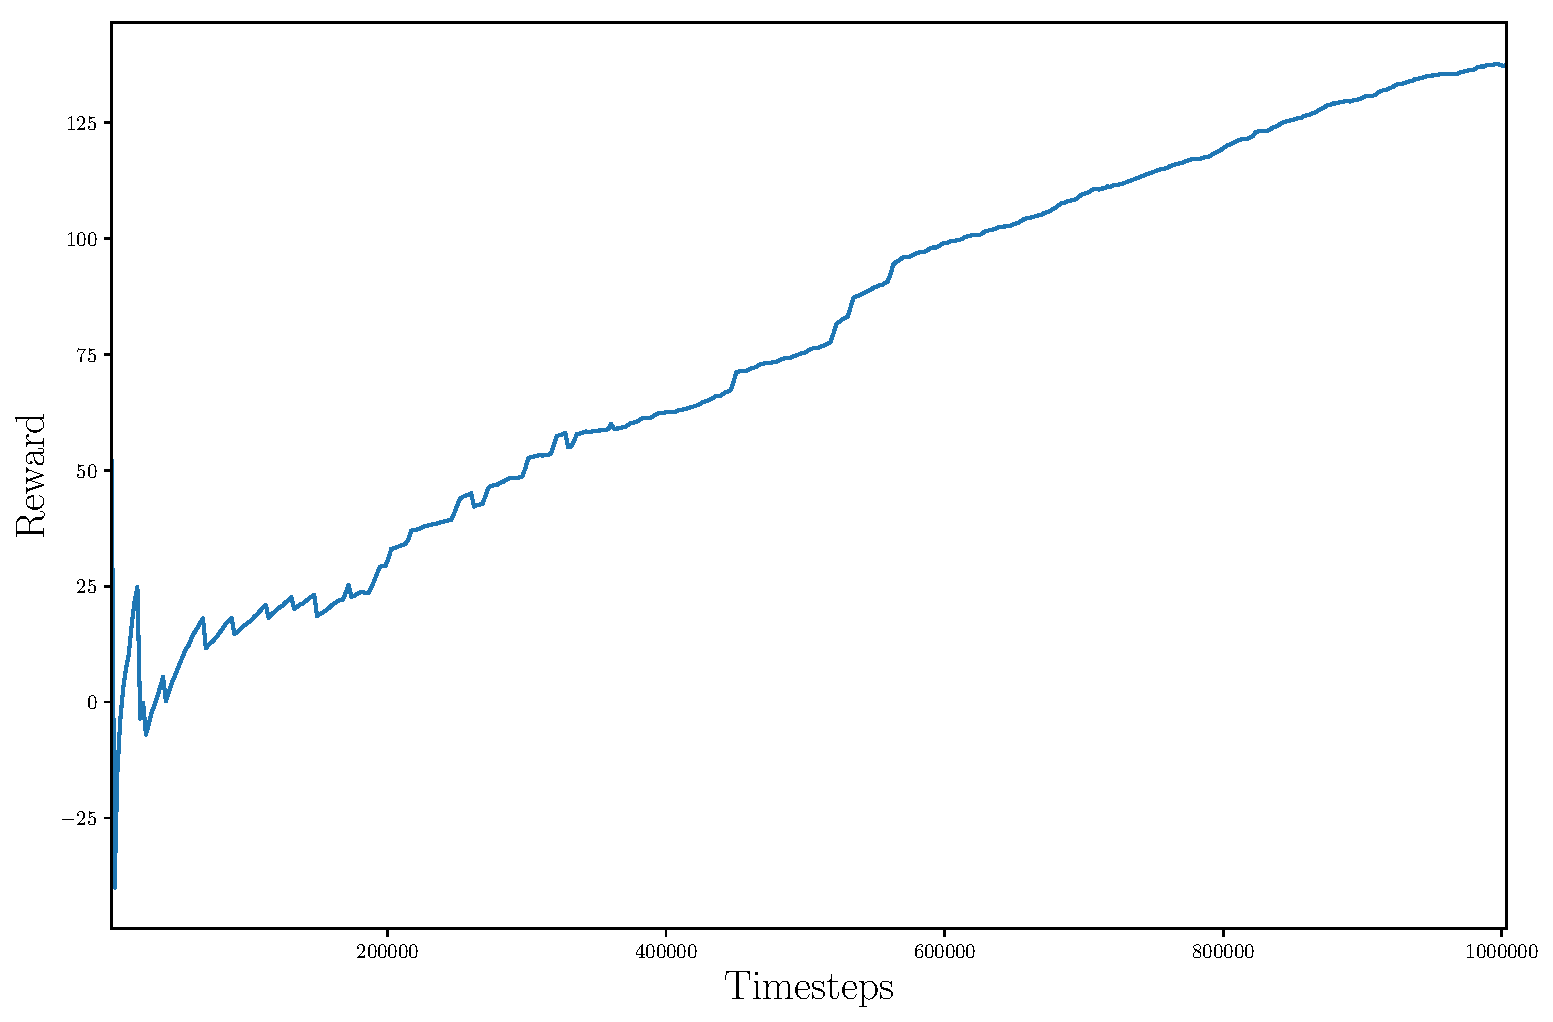
\includegraphics[width=0.9\textwidth]{Chapter7/ep_rew_walker.pdf}
	\caption{Episode Reward for the Constant Speed Walker task trained with PPO.}
	\label{fig:constant_episode_rew}
\end{figure}

In this task, the episode terminates early if the robot falls, therefore, measuring the episode duration
is also a good indicator of how stable the robot's current behavior is.
Figure \ref{fig:constant_episode_len} shows how the episode duration changes during training.
We see that the episode duration increases over training, which means that the agent is progressively
learning how to avoid falling.

\begin{figure}[ht]
	\centering
	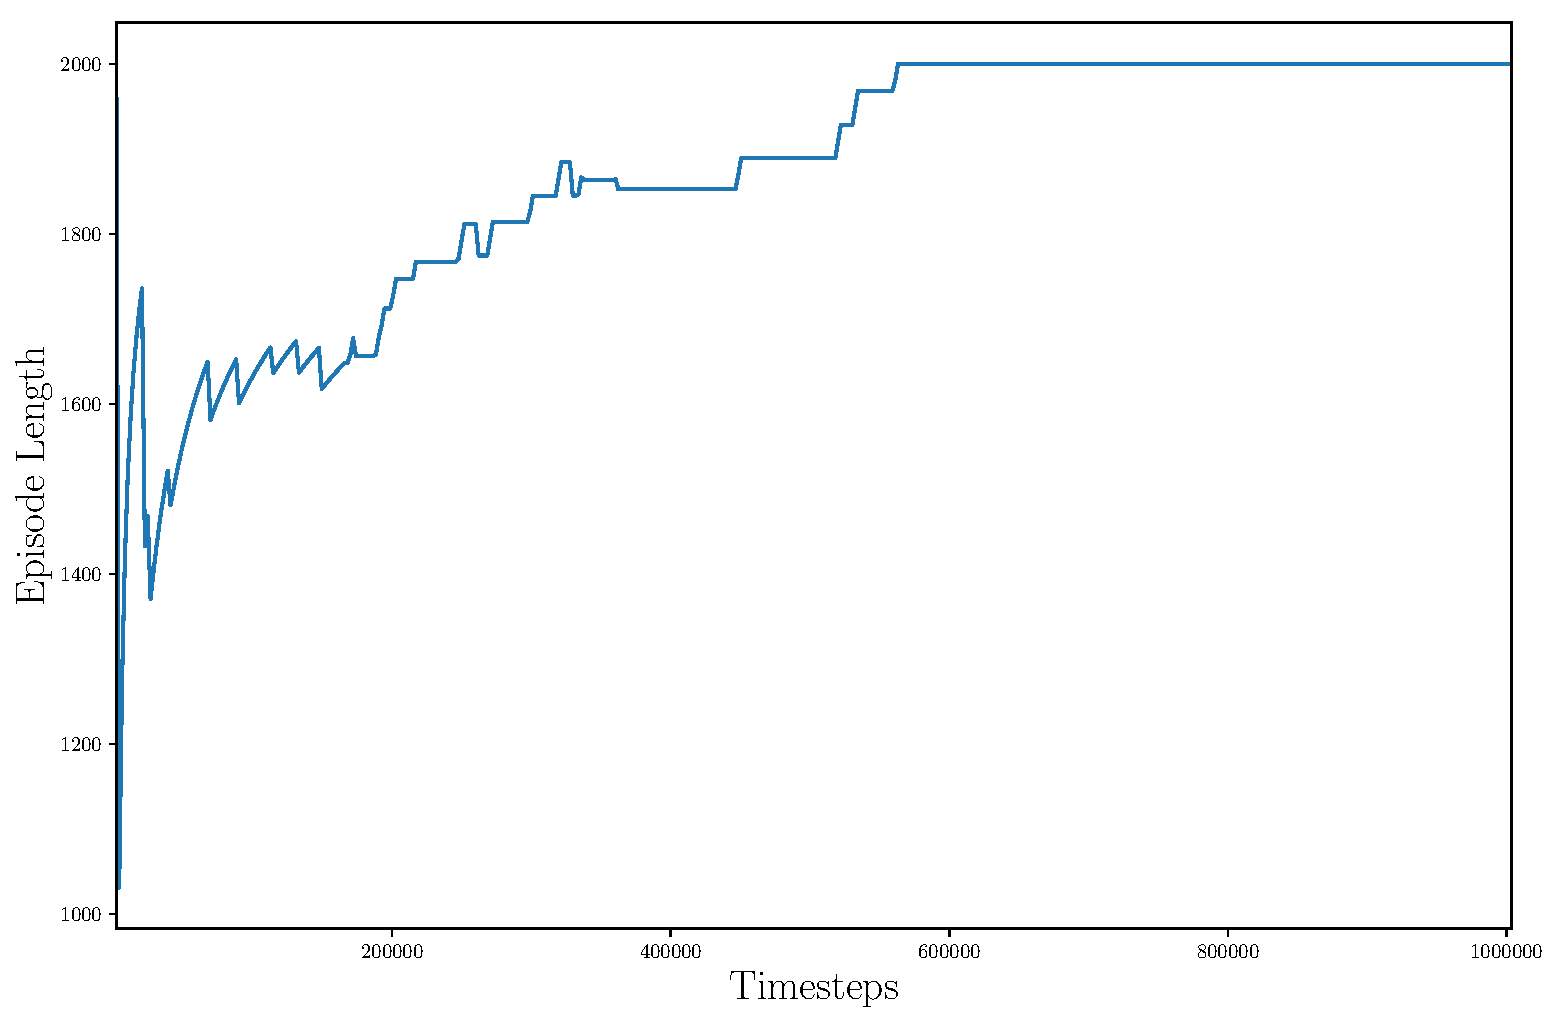
\includegraphics[width=0.9\textwidth]{Chapter7/ep_len_walker.pdf}
	\caption{Episode length for the Constant Speed Walker task with PPO.}
	\label{fig:constant_episode_len}
\end{figure}

Based on the results from Figure \ref{fig:constant_episode_rew} and \ref{fig:constant_episode_len}
we conclude that the agent is effectively learning how to walk with constant speed.
Since this is a very basic task, we chose not to use a baseline agent.

\section{Humanoid Racing Task}

In this domain, we ran PPO, TRPO and DDPG during $10^6$ timesteps with the parameters described in Appendix
\ref{chap:appendix_experiment}. We were interested in comparing the performance of these algorithms in this domain
to see which algorithms performs best in this task.
On average, each experiment took around $3$ hours to run.

Since the algorithms are stochastic and the server simulation is noisy and prone to numerical errors, 
we ran the experiments $5$ times for each algorithm and use the performance mean and standard deviation over all runs
to obtain more statistical significant results.
Figure \ref{fig:racer_episode_rew} depicts the episode rewards during the training phase for all runs. 
The dark line represents the reward mean and the transparent filling is the standard deviation
of all the executions.
Similarly, Figure \ref{fig:racer_episode_len} illustrates the mean of the episode reward length $\pm$ the standard deviation
over the same five runs.
\begin{figure}[ht]
	\centering
	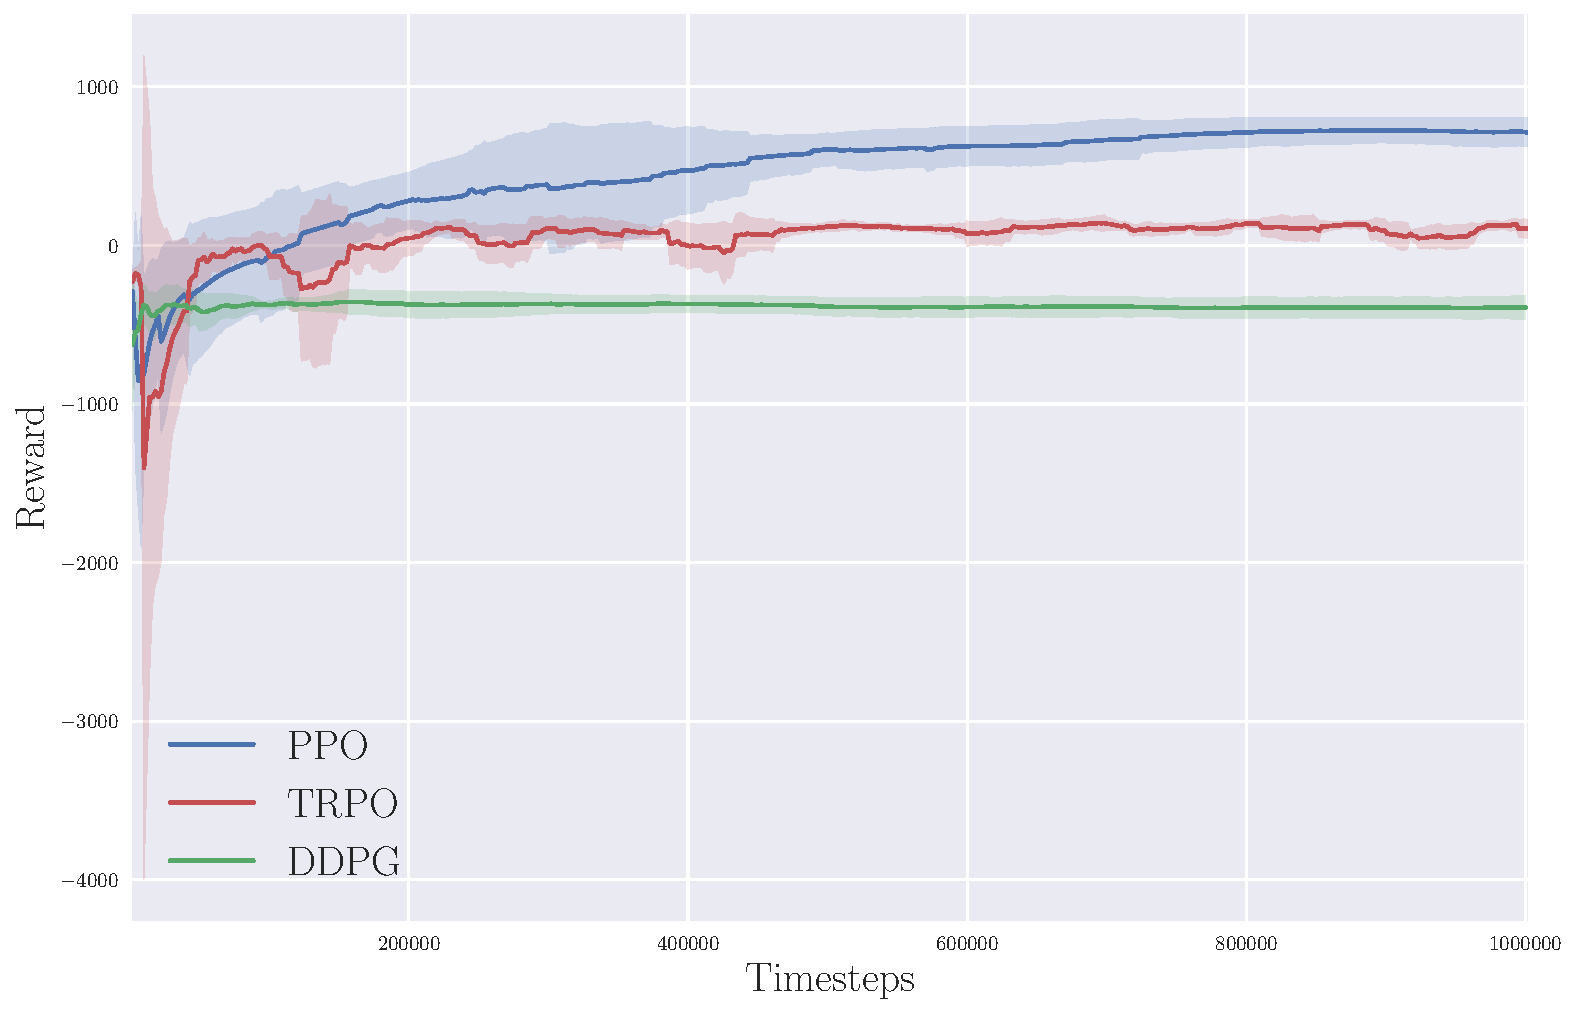
\includegraphics[width=0.9\textwidth]{Chapter7/reward.pdf}
	\caption{Average reward for PPO, TRPO and DDPG in the Racer task during training.
	The dark line is the mean over the $5$ runs and the transparent filling is
	 the standard deviation in regards to the mean.}
	\label{fig:racer_episode_rew}
\end{figure}

\begin{figure}[ht]
	\centering
	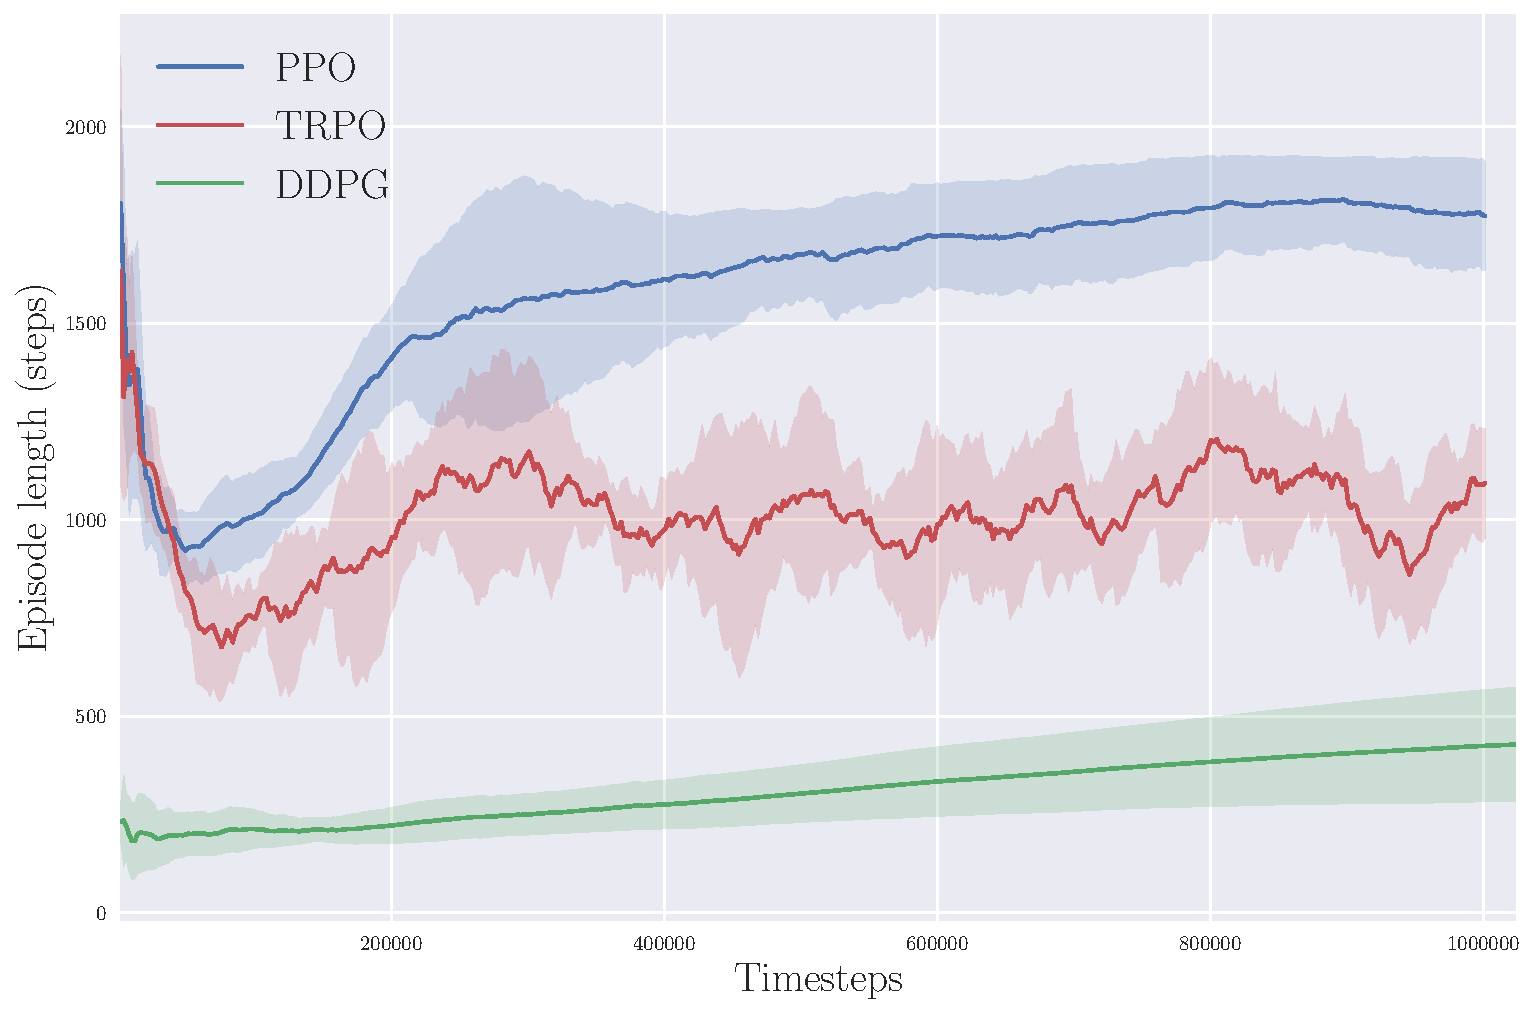
\includegraphics[width=0.9\textwidth]{Chapter7/episode_length.pdf}
	\caption{Episode length for PPO, TRPO and DDPG in the Racer task during training.
	The dark line is the mean over the $5$ runs and the transparent filling is
	the standard deviation in regards to the mean.}
	\label{fig:racer_episode_len}
\end{figure}

Figures and \ref{fig:racer_episode_rew} and \ref{fig:racer_episode_len} clearly show that 
the performance of PPO is consistently better than DDPG and TRPO for the racer task.
It is important to note that in the first $200000$ timesteps, the episode length for PPO and
TRPO are below the episode length at the end of training.
This means that, initially, that the robot is constantly falling down or leaving the race track until
it starts to learn that a better policy is to avoid falling and to stay on track, so the episodes
progressively take longer to terminate.
We also point out that the DDPG agent barely improves over time.

During the evaluation phase, we observe that the only agent that actually reaches the finish line was the 
robot trained using PPO. 
We chose one of the learned policies and used it to compare against an open loop ``go-straight" controller
that simply goes straight.
We analyse 20 trajectories executed by the PPO learned policy and compare them with those executed by the baseline.
The results are show in Figure \ref{fig:trajectory}.

\begin{figure}[b]
	\centering
	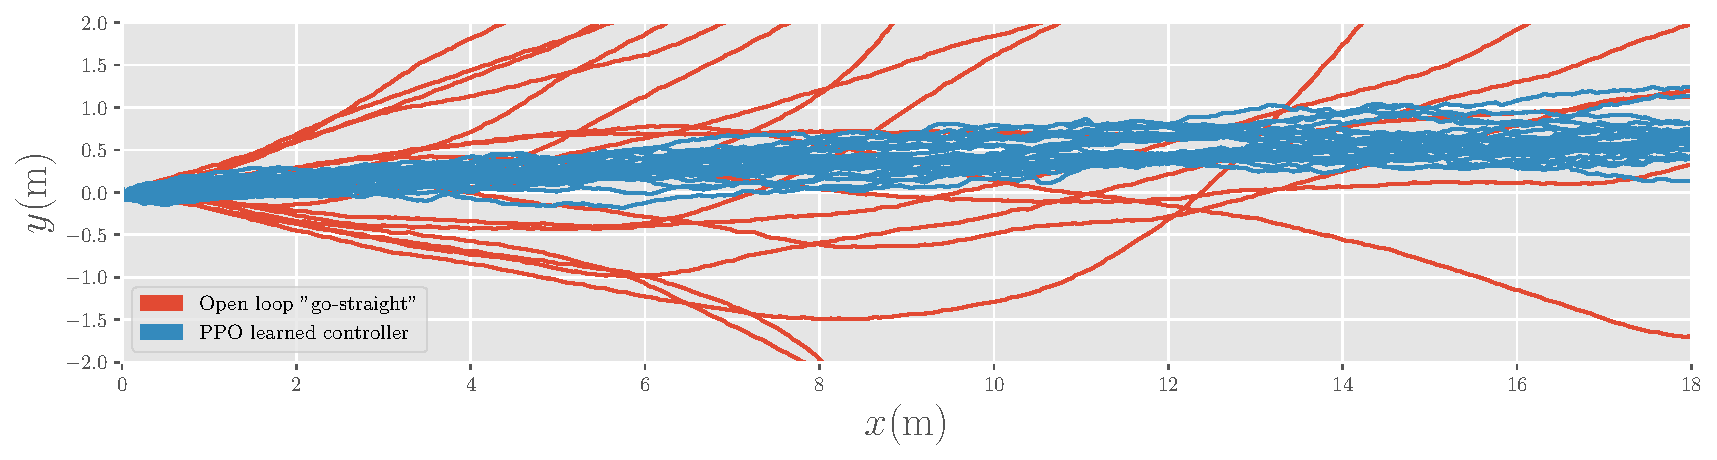
\includegraphics[width=1\textwidth]{Chapter7/trajectory.pdf}
	\caption{Trajectories comparison between one of the trained PPO controllers and the open loop ``go-straight" controller.}
	\label{fig:trajectory}
\end{figure}

For these trajectories, the empirical results can be summarized as follows: 

\begin{itemize}
	\item \textbf{Total race average speed} $\overline{v_x} \approx 0.6$ m/s. The speed expresses how fast, on average,
	the agent completed the race. Notice that the walking engine's stability constraints limits the robot's
	speed to approximately $0.9$ m/s. Therefore, in comparison to both the baseline - that rarely finishes the task - and
	theoretical fastest policy, the learned policy does very well on this task.
	\item \textbf{Horizontal displacement average} $y_{\text{mean}} \approx 0.47$ m. This represents how far,
	horizontally, from to the center line of the race track, the agent finishes the race. Since the race track
	is 4m wide, the average horizontal displacement is small as shown in Figure \ref{fig:trajectory}.
	Note that the robot did not leave the race track in all $20$ trajectories.
\end{itemize}

These results show that the robot successfully learned how to complete the task, performing significantly better
than the baseline.
However, we also observe that this policy was a bit biased in regards to the horizontal displacement
and therefore could still be further improved.

\section{Humanoid Soccer Dribbling Task}

In this problem, we ran PPO, TRPO and DDPG during $1.7\text{x} 10^6$ timesteps with the parameters described in Appendix
\ref{chap:appendix_experiment}. In comparison with the other tasks, learning to dribble
requires much more data since it is a far more challenging task.
We compare the performance of these algorithms and analyse how well the learned policy does in comparison to
the baseline dribble behavior implemented by the ITAndroids team.
On average, each experiment took much longer to run, around $8$ hours per experiment.
The main reason for this is that there is an additional simulation robot that
interacts with the environment. 
This was very challenging, since this made the process of iterating over different approaches much slower.

Similarly to the previous task, 
we ran the experiments $5$ times for each algorithm and calculated the performance mean and standard deviation over all runs.
Figure \ref{fig:dribbling_episode_rew} depicts the episode rewards during the training phase for all runs. 
The dark line represents the reward mean and the transparent filling is the standard deviation
of all the executions.

\begin{figure}[h]
	\centering
	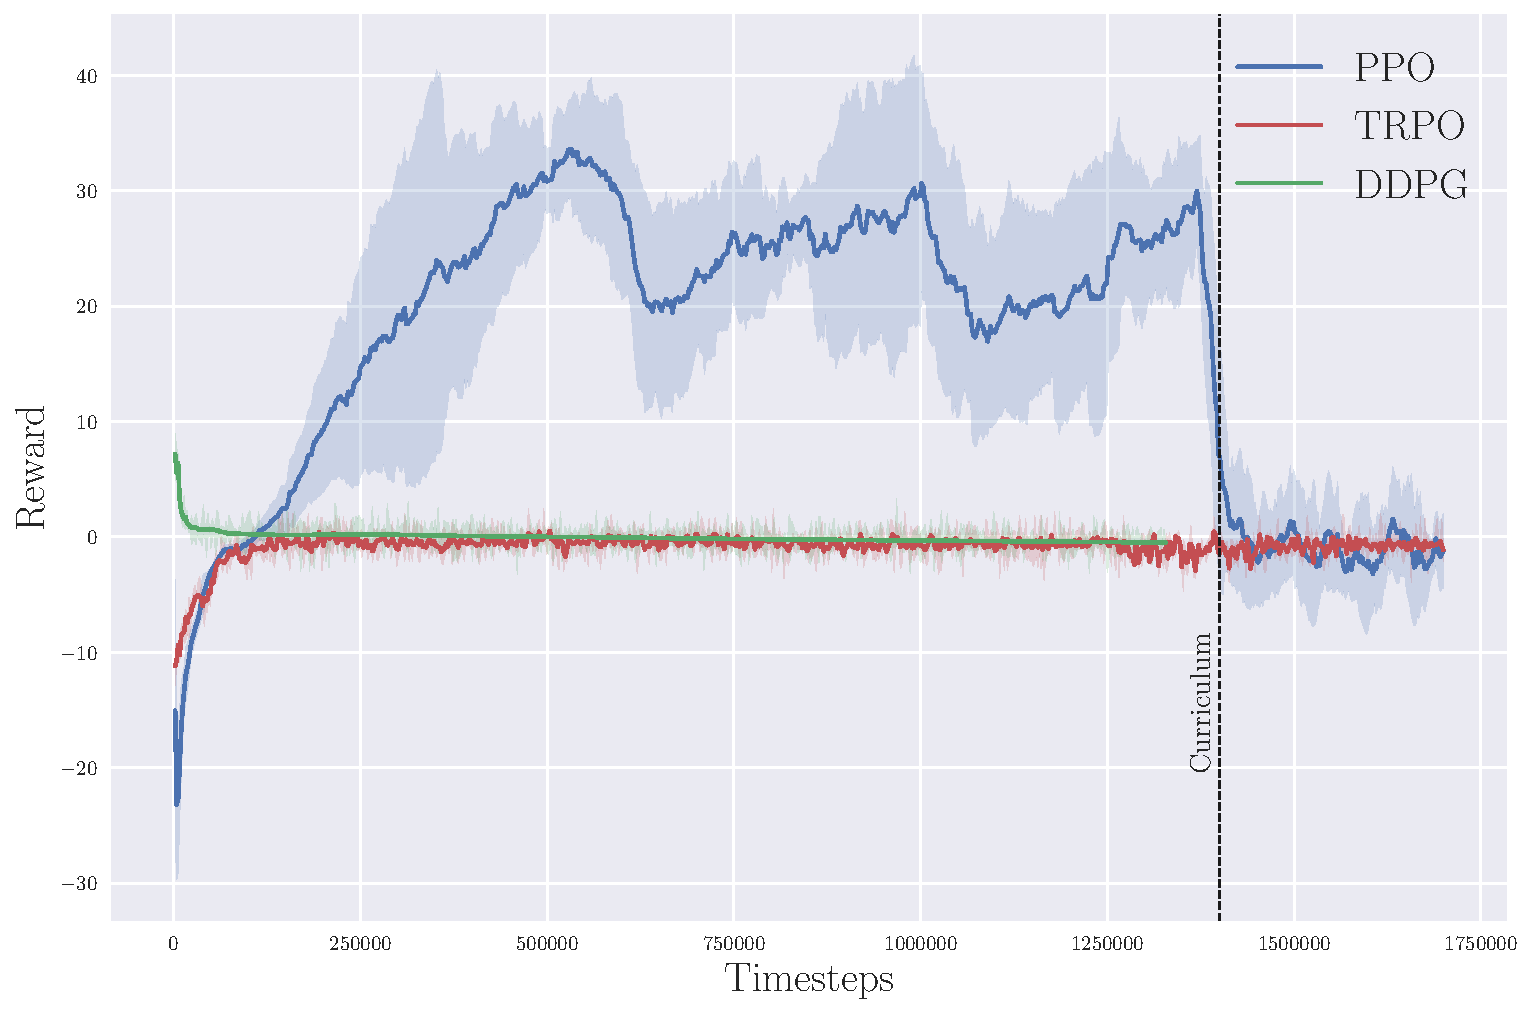
\includegraphics[width=0.9\textwidth]{Chapter7/dribbling/Reward.pdf}
	\caption{Average reward for PPO, TRPO and DDPG in the dribbling task during training.
	The dark line is the mean over the $5$ runs and the transparent filling is
	 the standard deviation in regards to the mean and the doted line represents when the curriculum changes.}
	\label{fig:dribbling_episode_rew}
\end{figure}

For PPO, we notice a sharp drop in the average reward when the curriculum changes.
This is expected since a better opponent makes it harder for the learning agent to complete the dribble
(and get more reward). Furthermore, not all agents are able to successfully learn to dribble since the 
average rewards for some agents are negative.
Similarly, Figure \ref{fig:dribbling_episode_len} illustrates episode length mean $\pm$ the standard deviation
over the same five runs.

\begin{figure}[h]
	\centering
	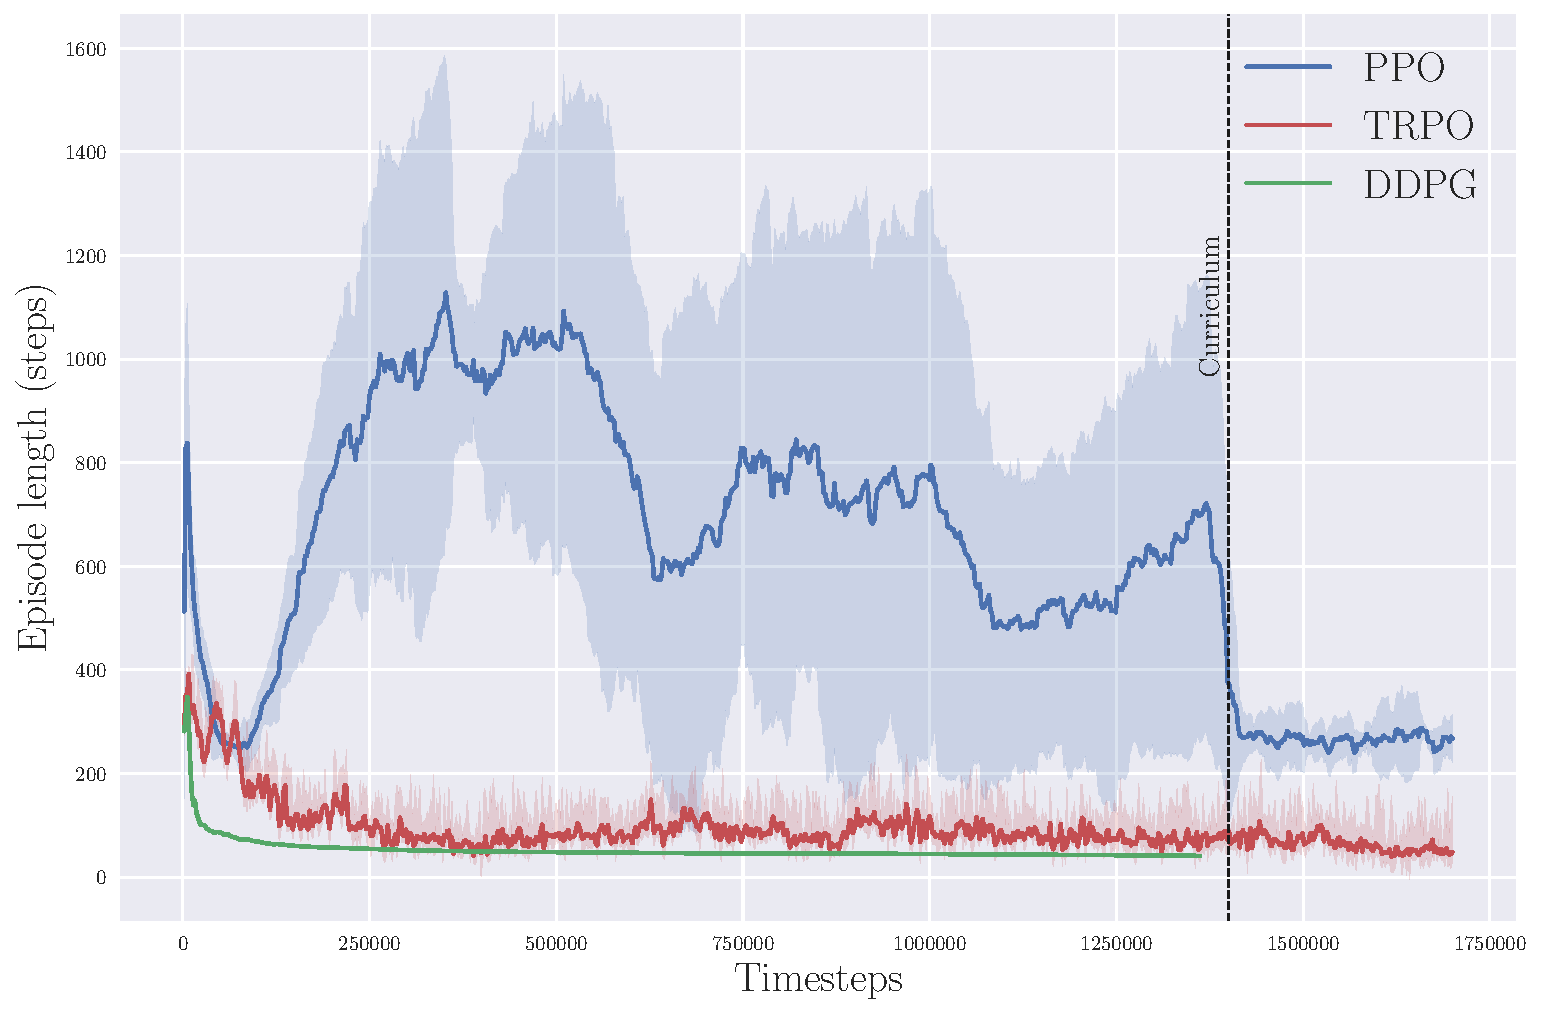
\includegraphics[width=0.9\textwidth]{Chapter7/dribbling/Episodelength(steps).pdf}
	\caption{Episode length for PPO, TRPO and DDPG in the dribbling task during training.
	The dark line is the mean over the $5$ runs and the transparent filling is
	the standard deviation in regards to the mean and the doted line represents when the curriculum changes.}
	\label{fig:dribbling_episode_len}
\end{figure}

We notice a similar sharp drop in the episode duration when the curriculum changes. This is also
expected since the agent must learn to dribble faster to avoid losing the ball to the opponent.
Furthermore, the average reward has a higher variance in comparison to the previous task.
This could mean that the policy space of successful dribbling policies is higher than for the
previous task since the task is significantly more complex.

% Figures and \ref{fig:racer_episode_rew} and \ref{fig:racer_episode_len} clearly show that 
% the performance of PPO is consistently better than DDPG and TRPO for the racer task.
% It is important to note that in the first $200000$ timesteps, the episode length for PPO and
% TRPO are below the episode length at the end of training.
% This means that, initially, that the robot is constantly falling down or leaving the race track until
% it starts to learn that a better policy is to avoid falling and staying on track and the episodes
% progressively take longer to terminate.
% We also point out that the DDPG agent barely improves over time.

To evaluate our results, we chose one of the learned policies and ran this task for $2000$ episodes
against the ITAndroids baseline agent.
We used metric $M$ for measuring how good the agent performed on the task and is given by the rate of successful dribbles,
defined in Equation \ref{eq:metric}.

\begin{equation}
	M = \dfrac{N_{\text{agent dribbles}}}{N_{\text{agent dribbles}} + N_{\text{opp dribbles}}}
	\label{eq:metric}
\end{equation}
where $N_{\text{agent dribbles}}$ is the number of successful dribbles by the agent and
$N_{\text{agent dribbles}}$ is number of successful dribbles by the opponent.
We considered a successful dribble when an agent managed to move the ball
out of the task region, towards its attacking side.
We also calculated how long, on average, each robot takes to complete the dribble.

The results are summarized in Table \ref{tab:dribble}

\begin{table}[ht]
    \begin{tabular}{|l|l|l|}
    \hline
    Agent            &Successful dribble rate ($M$)   & Average dribble duration (in timesteps) \\ \hline
    Learning Agent   &$ 68.2$\%                       & $298.2$               \\
    Baseline Agent   &$ 31.8$\%                       & $321.6$                \\ \hline
    \end{tabular}
\centering
\caption{Evaluation results of the dribbling task.}
\label{tab:dribble}
\end{table}

We can see that the learned agent greatly outperforms the baseline, despite taking longer on average
to complete the task.
A video of the trained agent executing the task is available at the GitHub repository.
